\documentclass[10pt]{beamer}
\usetheme{CambridgeUS}
\usecolortheme{dolphin}
\usepackage{preamble}


\def\Ra{\mathrm{Ra}}
\def\Pr{\mathrm{Pr}}
\def\Le{\mathrm{Le}}

% set colors
\definecolor{myNewColorA}{RGB}{124, 13,14}
\definecolor{myNewColorB}{RGB}{124, 13,14}
\definecolor{myNewColorC}{RGB}{124, 13,14} % {130,138,143}
\setbeamercolor*{palette primary}{bg=myNewColorC}
\setbeamercolor*{palette secondary}{bg=myNewColorB, fg = white}
\setbeamercolor*{palette tertiary}{bg=myNewColorA, fg = white}
\setbeamercolor*{titlelike}{fg=myNewColorA}
\setbeamercolor*{title}{bg=myNewColorA, fg = white}
\setbeamercolor*{item}{fg=myNewColorA}
\setbeamercolor*{caption name}{fg=myNewColorA}
\usefonttheme{professionalfonts}


% Set the block color
\setbeamercolor{block title}{bg=myNewColorA, fg=white} % Block title color
\setbeamercolor{block body}{bg=myNewColorA!10} % Block body color
% % Adjust the size of the block
\setbeamertemplate{blocks}[rounded][shadow=true] % Rounded corners and shadow
% \addtobeamertemplate{block begin}{\begin{adjustbox}{width=\textwidth}}{\end{adjustbox}}
% \addtobeamertemplate{block end}{\end{adjustbox}}{}
%gets rid of bottom navigation bars
\setbeamertemplate{footline}[frame number]{}

%gets rid of bottom navigation symbols
\setbeamertemplate{navigation symbols}{}



\title{Thermohaline circulation}
\author{Víctor Ballester and Victor Botez}
\institute{\centering
Computational Fluid Dynamics\endgraf
M2 - Applied and Theoretical Mathematics\endgraf
Université Paris-Dauphine, PSL}
\date{April 4, 2024}


%------------------------------------------------------------
%This block of commands puts the table of contents at the 
%beginning of each section and highlights the current section:
%\AtBeginSection[]
%{
%  \begin{frame}
%    \frametitle{Contents}
%    \tableofcontents[currentsection]
%  \end{frame}
%}
\AtBeginSection[]{
  \begin{frame}
  \vfill
  \centering
  \begin{beamercolorbox}[sep=8pt,center,shadow=true,rounded=true]{title}
    \usebeamerfont{title}\insertsectionhead\par%
  \end{beamercolorbox}
  \vfill
  \end{frame}
}
% ------Contents below------
%------------------------------------------------------------

\begin{document}

%The next statement creates the title page.
\frame{\titlepage}

\begin{frame}{Table of contents}
  \tableofcontents
\end{frame}

\section{Introduction}

\begin{frame}{Motivation}
  \begin{itemize}
    \item Thermohaline circulation is a global circulation of the ocean that is driven by the density differences due
          to temperature and salinity.
    \item It is responsible for the transport of heat and salt around the globe, and it plays a key role in the climate system.
  \end{itemize}
  \begin{figure}
    \centering
    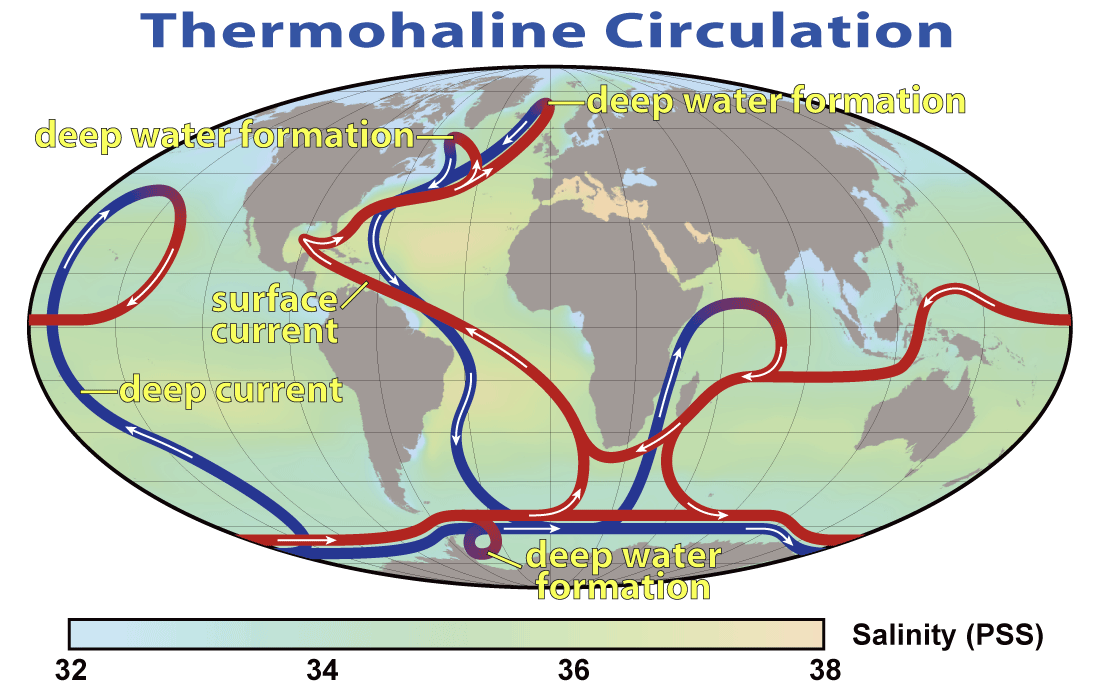
\includegraphics[width=0.5\textwidth]{images/Thermohaline_Circulation_2.png}
    \caption{Schematic of the thermohaline circulation.}
  \end{figure}

\end{frame}
\begin{frame}{Objectives}
  Our goals are:
  \begin{itemize}
    \item Study the thermohaline circulation in a two-dimensional domain.
    \item Analyze the stability of the convection patterns.
    \item Investigate the impact of the initial conditions on the convection patterns.
  \end{itemize}
\end{frame}

\section{Theoretical model}
    

\begin{frame}{Governing equations (I)}
Navier-Stokes equations and diffusion equations for salinity and temperature :
\begin{equation}
  \begin{aligned}
    \rho\left(\frac{\partial\mathbf{u}}{\partial t} + (\mathbf{u}\cdot\nabla)\mathbf{u}\right) & = -\nabla P + \rho\nu\nabla^2\mathbf{u} + \rho \mathbf{g} \\
    \pdv{\rho}{t} + \nabla\cdot(\rho\mathbf{u})                                                & = 0                                                       \\
    \frac{\partial T}{\partial t} + (\mathbf{u}\cdot\nabla)T                                   & = \kappa_T \nabla^2T                                      \\
    \frac{\partial S}{\partial t} + (\mathbf{u}\cdot\nabla)S                                   & = \kappa_S \nabla^2S                                      \\
  \end{aligned}
\end{equation}
Taylor expansion of density :
\begin{equation}
  \rho = \rho_0(1-\alpha_T\Delta T + \alpha_S\Delta S)
\end{equation}


\end{frame}

\begin{frame}{Governing equations (II)}
Navier-Stokes equations :
\begin{equation}
  \begin{aligned}
    \left(\frac{\partial\mathbf{u}}{\partial t} + (\mathbf{u}\cdot\nabla)\mathbf{u}\right) & = -\frac{\nabla P}{\rho _0} + \nu\nabla^2\mathbf{u} + \rho_0\left(\alpha_T \Delta T - \alpha_S \Delta S \right) g\mathbf{e_z} \\
    \nabla\cdot\mathbf{u}& = 0  \end{aligned}
\end{equation}
Diffusion equations :
\begin{equation}
    \begin{aligned}
        \frac{\partial T}{\partial t} + (\mathbf{u}\cdot\nabla)T                                   & = \kappa_T \nabla^2T                                      \\
    \frac{\partial S}{\partial t} + (\mathbf{u}\cdot\nabla)S                                   & = \kappa_S \nabla^2S                                      \\    
    \end{aligned}
\end{equation}


\end{frame}
\begin{frame}{Boundary conditions}
\begin{figure}[ht]
  \centering
  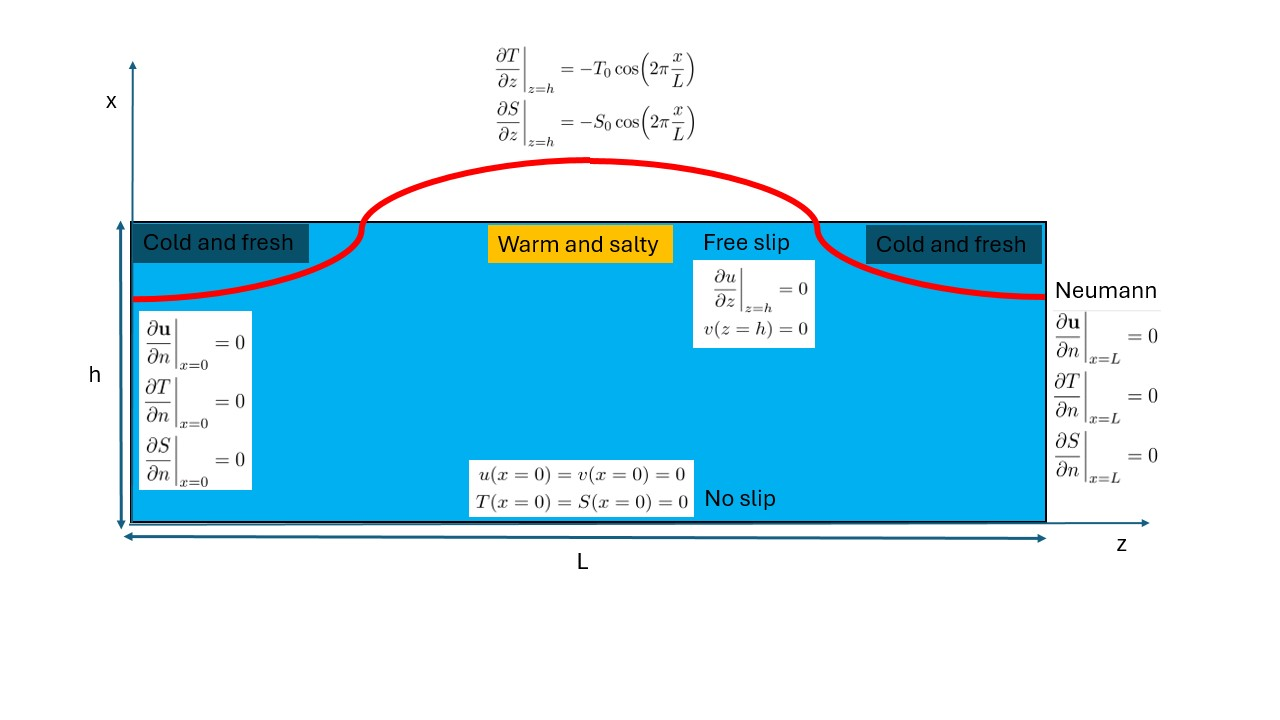
\includegraphics[width=1.\textwidth]{images/drawing_setup.jpg}
  \caption{Drawing of the setup used in all simulations.}
  \label{fig:setup}
\end{figure}
\end{frame}

\begin{frame}{Dimensionless equations and control parameters}
Navier-Stokes equations in the Boussinesq approximation :
\begin{equation}\label{eq:ns}
  \begin{aligned}
    \frac{\partial\mathbf{u}}{\partial t} + (\mathbf{u}\cdot\nabla)\mathbf{u} & = -\nabla p + \Pr\nabla^2\mathbf{u} + \Pr\Ra\left(T - \frac{1}{R_{\rho}}S\right)\vf{e}_z \\
    \frac{\partial T}{\partial t} + (\mathbf{u}\cdot\nabla)T                  & = \nabla^2T                                                                              \\
    \frac{\partial S}{\partial t} + (\mathbf{u}\cdot\nabla)S                  & = \frac{1}{\Le}\nabla^2S                                                                 \\
    \nabla\cdot\mathbf{u}                                                     & = 0
  \end{aligned}
\end{equation}
Dimensionless quantities : 
\begin{equation}
    \Pr = \frac{\nu}{\kappa_T}
\end{equation}
\begin{equation}
    \Ra = \frac{\alpha_T g T_0 h^3}{\nu \kappa_T}
\end{equation}
\begin{equation}
    R_{\rho} = \frac{\alpha_T T_0}{\alpha_S S_0}
\end{equation}
\begin{equation}
    \Le = \frac{\kappa_T}{\kappa_S}
\end{equation}
\end{frame}

\section{Numerical methods}

\begin{frame}{Chorin splitting method}
  In order to integrate the incompressible Navier-Stokes equations, we use the Chorin splitting method:
  \begin{enumerate}
    \item Solve for $\vf{u}^a$ in $\displaystyle  \frac{\vf{u}^a-\vf{u}^n}{\Delta t} + \vf{u}^n \cdot \nabla \vf{u}^n = 0$ using a semi-Lagrangian method.
    \item Solve for $\vf{u}^*$ in $\displaystyle  \frac{\vf{u}^* - \vf{u}^a}{\Delta t} = \Pr \nabla^2 \vf{u}^n +\Pr\Ra\left(T^n - \frac{1}{R_{\rho}}S^n\right)\vf{e}_z$ using a central differences scheme.
    \item Set the boundary conditions for the intermediate velocity field $\vf{u}^*$.
    \item Solve the Poisson equation for the pressure, $\displaystyle \nabla^2 p^{n+1} = \frac{1}{\Delta t}\nabla \cdot \vf{u}^*$.
    \item Set the boundary conditions for the pressure $p^{n+1}$.
    \item Project the pressure to the intermediate velocity to obtain the new velocity at time $t^{n+1}$, $\displaystyle \vf{u}^{n+1} = \vf{u}^* - \Delta t\nabla p^{n+1}$.
    \item Set the boundary conditions for the velocity field $\vf{u}^{n+1}$.
  \end{enumerate}
\end{frame}

\begin{frame}{Temperature and salinity evolutions}
  For each time step, once we gave found the next iterate of the velocity field $\vf{u}^{n+1}$, we solve the advection-diffusion equations for the temperature and salinity fields:
  \begin{enumerate}
    \item Solve for $T^{a}$ in $\displaystyle  \frac{T^{a}-T^{n}}{\Delta t} + \vf{u}^{n+1} \cdot \nabla T^{n} = 0$ and for $S^{a}$ in $\displaystyle  \frac{S^{a}-S^{n}}{\Delta t} + \vf{u}^{n+1} \cdot \nabla S^{n} = 0$ using a semi-Lagrangian method.
    \item Solve for $T^{n+1}$ in $\displaystyle  \frac{T^{n+1}-T^{a}}{\Delta t} = \nabla^2 T^{n}$ and for $S^{n+1}$ in $\displaystyle  \frac{S^{n+1}-S^{a}}{\Delta t} = \frac{1}{\Le}\nabla^2 S^{n}$ using a central differences scheme.
    \item Set the boundary conditions for the temperature and salinity fields $T^{n+1}$ and $S^{n+1}$.
  \end{enumerate}
\end{frame}

\begin{frame}{Implicit vs explicit}
  Problems with the explicit method:
  \begin{itemize}
    \item The time step is limited by the stability condition of the heat equation $\partial_t f= \kappa\nabla^2 f$:
          $$
            \kappa\Delta t\left( \frac{1}{\Delta x^2} + \frac{1}{\Delta y^2} \right) \leq \frac{1}{2}.
          $$
    \item For us $\kappa = \Pr,1,\frac{1}{\Le}$, and for water $\Pr\sim 10$, which implies $\Delta t\leq 2.5\times 10^{-6}$ for $\Delta x=\Delta y=0.01$!
  \end{itemize}
  \vspace{0.5cm}
  \textbf{Solution:} use an implicit method for the heat equation to make it unconditionally stable!
  \begin{enumerate}
    \setcounter{enumi}{1}
    \item Solve for $\vf{u}^*$ in $\displaystyle  \frac{\vf{u}^* - \vf{u}^a}{\Delta t} = \Pr \nabla^2 \vf{u}^* +\Pr\Ra\left(T^n - \frac{1}{R_{\rho}}S^n\right)\vf{e}_z$ using a central differences scheme.
  \end{enumerate}
  Our scheme is still consistent because at zero order in time $\vf{u}^* = \vf{u}^{n+1}$.
\end{frame}

\begin{frame}{Boundary conditions and ghost points}
  We use the ghost cell method to impose second order boundary conditions to the actual boundary of the domain.
  \vspace{0.5cm}

  \begin{figure}
    \centering
    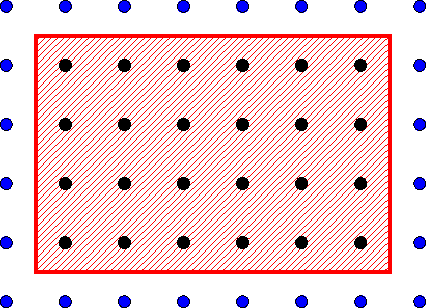
\includegraphics[width=0.5\textwidth]{images/grid.pdf}
    \caption{The ghost cell method. The domain is represented in red and the dots represent the grid cells, the black ones being the inner cells and the blue ones, the ghost cells.}
  \end{figure}

\end{frame}

\section{Results}

\begin{frame}{Convection phase diagram}
  \textbf{Aim:} fixed $\Pr$ and $\Ra$, study the convection patterns in terms of the $\Le$ (measures the ratio of diffusivities) and $R_{\rho}$ (measures the importance in the density).

  We focus our study on a neighbourhood of $R_{\rho} = 1$, where both temperature and salinity are equally important in the density. We do the study for $\Le\in \{0.01,0.1,1,10,100\}$.
  \begin{figure}
    \centering
    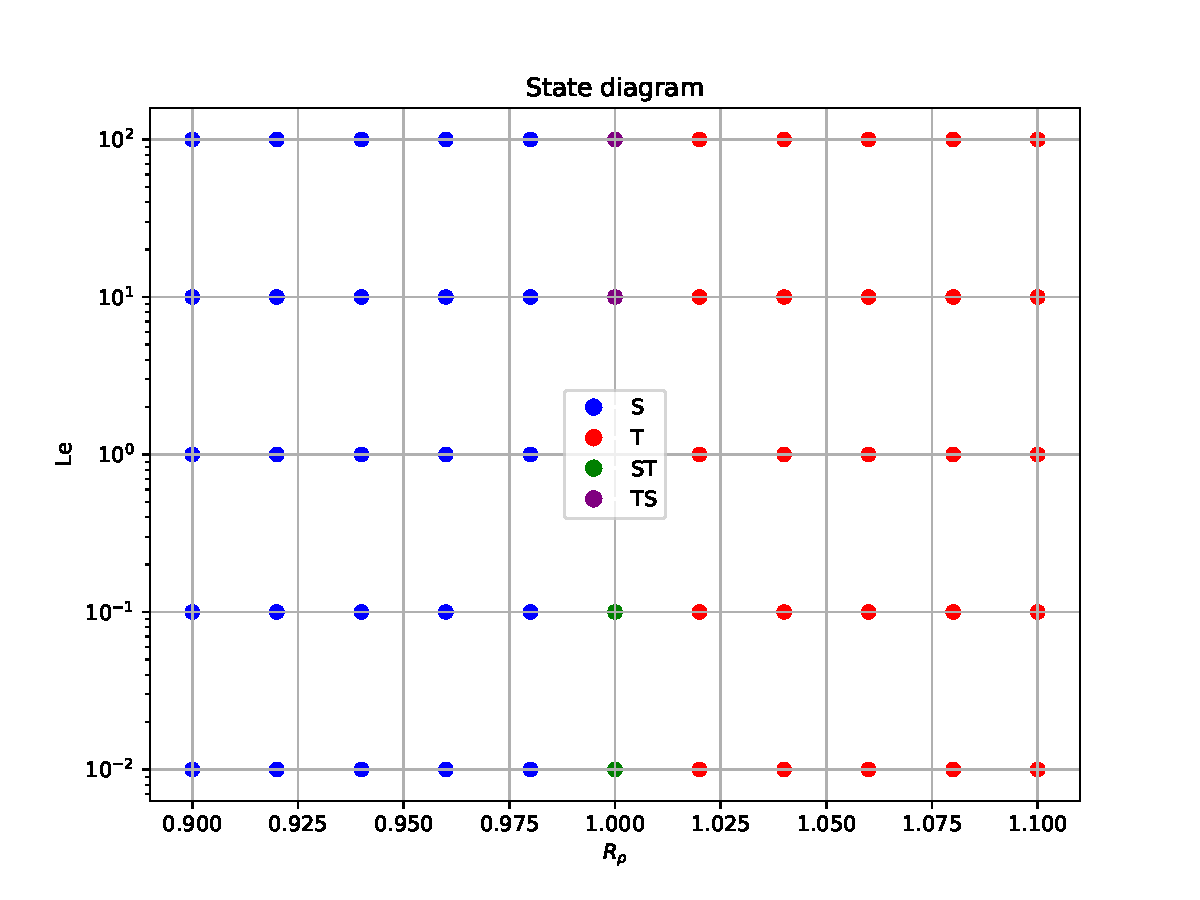
\includegraphics[width=0.5\textwidth]{images/phase_diagram.pdf}
    \caption{Phase diagram of the convection patterns.}
  \end{figure}


\end{frame}

\begin{frame}
  \begin{figure}[ht]
    \centering
    \begin{subfigure}{\textwidth}
      \centering
      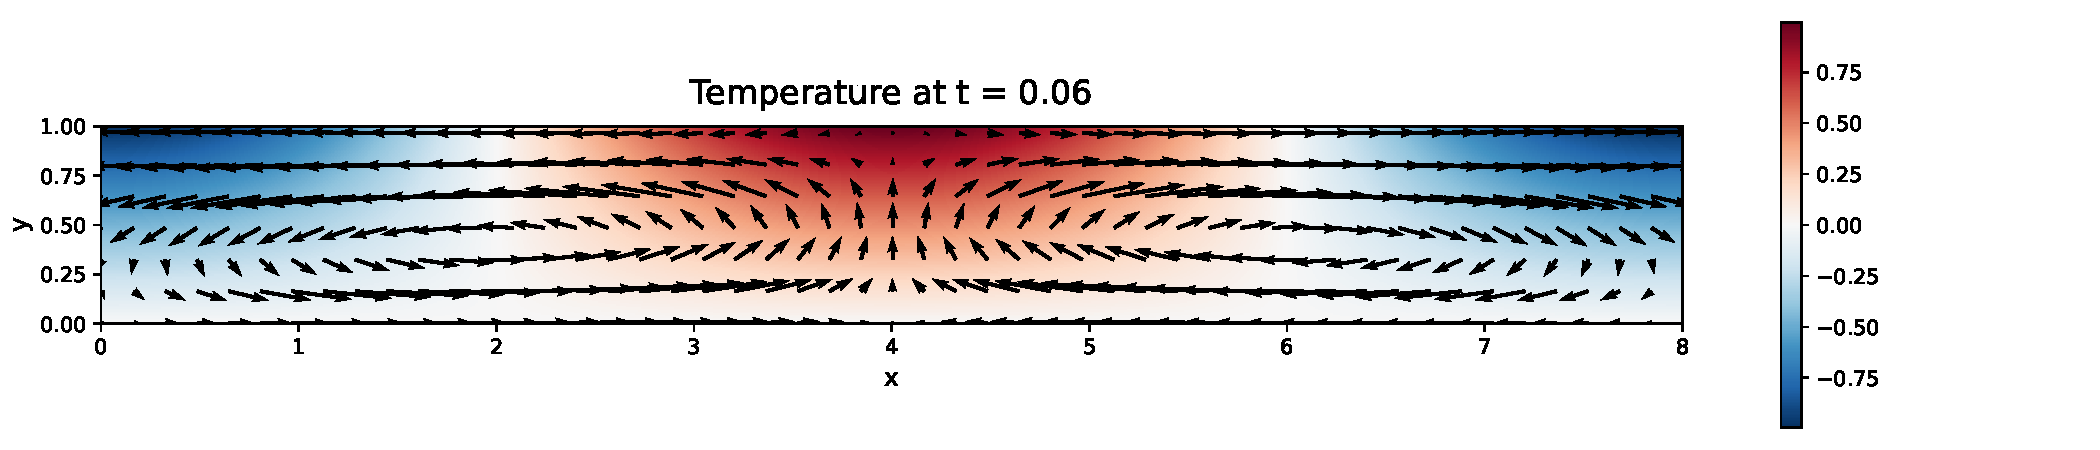
\includegraphics[width=0.75\textwidth]{images/TS_2.pdf}
    \end{subfigure}\\
    \begin{subfigure}{\textwidth}
      \centering
      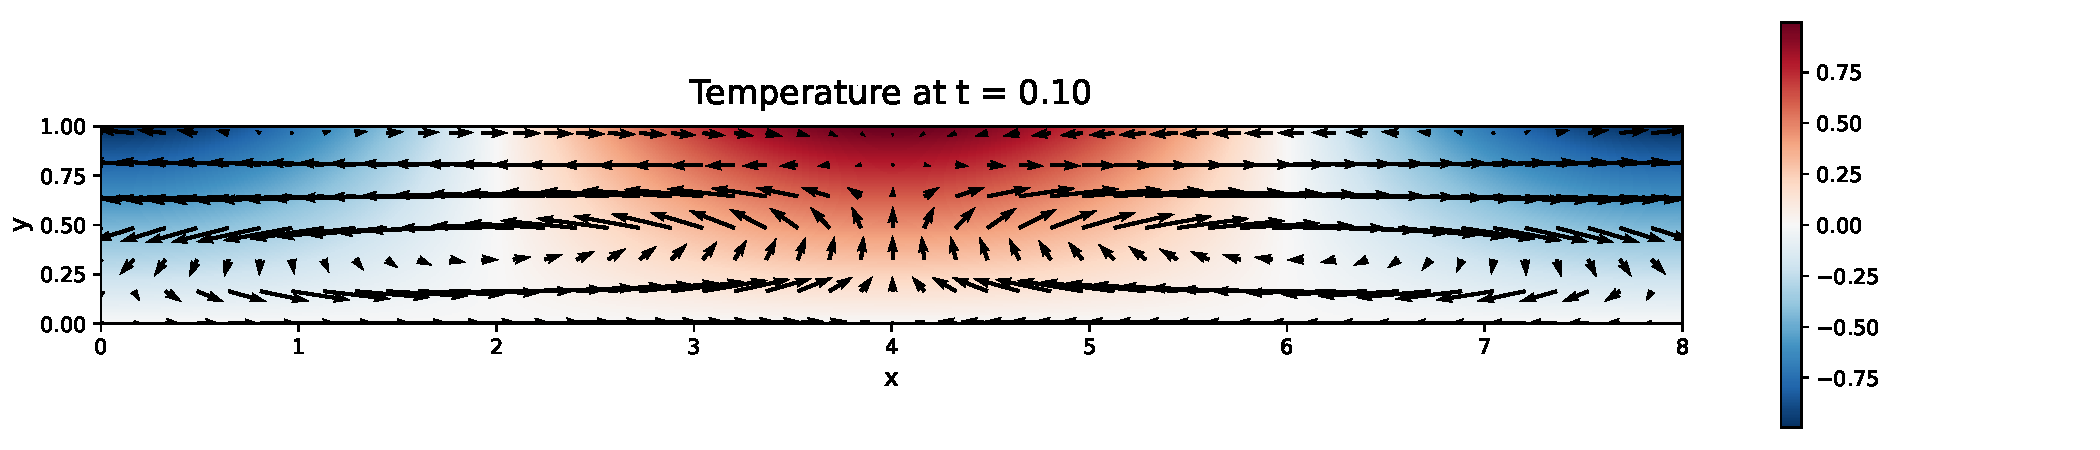
\includegraphics[width=0.75\textwidth]{images/TS_3.pdf}
    \end{subfigure}\\
    \begin{subfigure}{\textwidth}
      \centering
      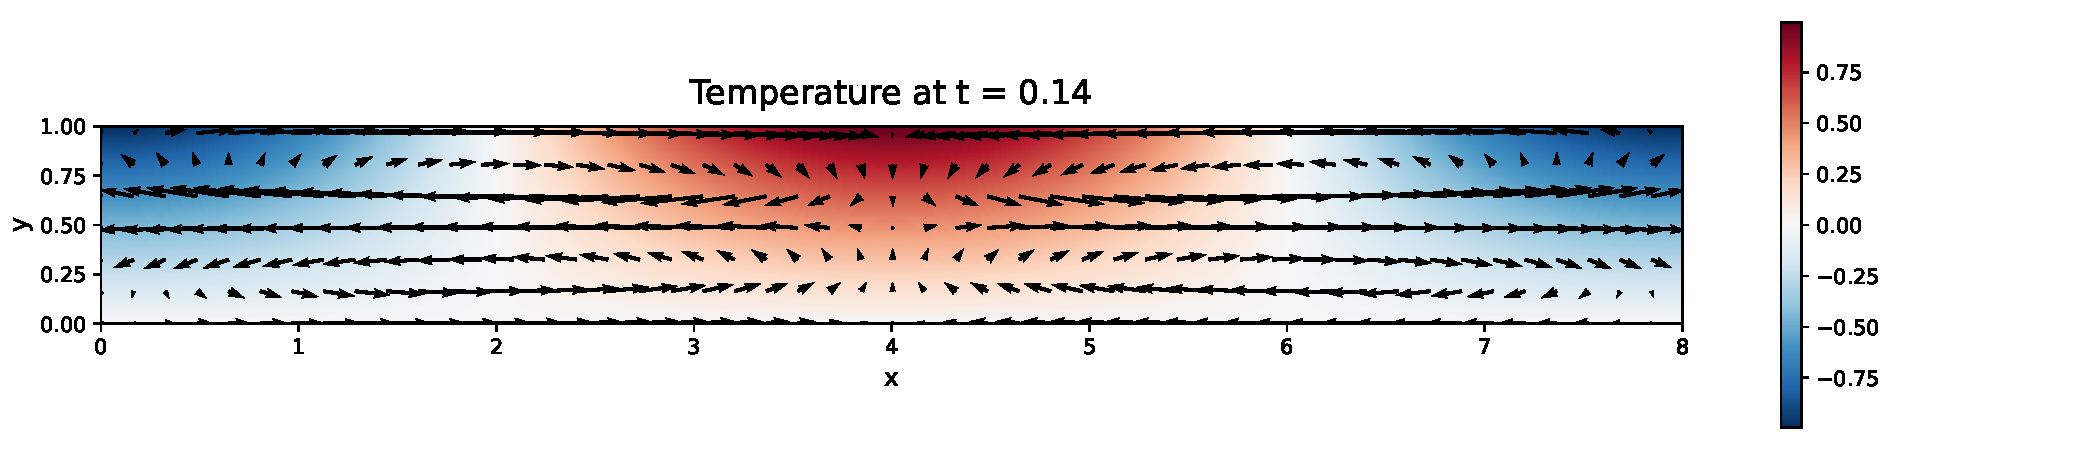
\includegraphics[width=0.75\textwidth]{images/TS_4.pdf}
    \end{subfigure}\\
    \begin{subfigure}{\textwidth}
      \centering
      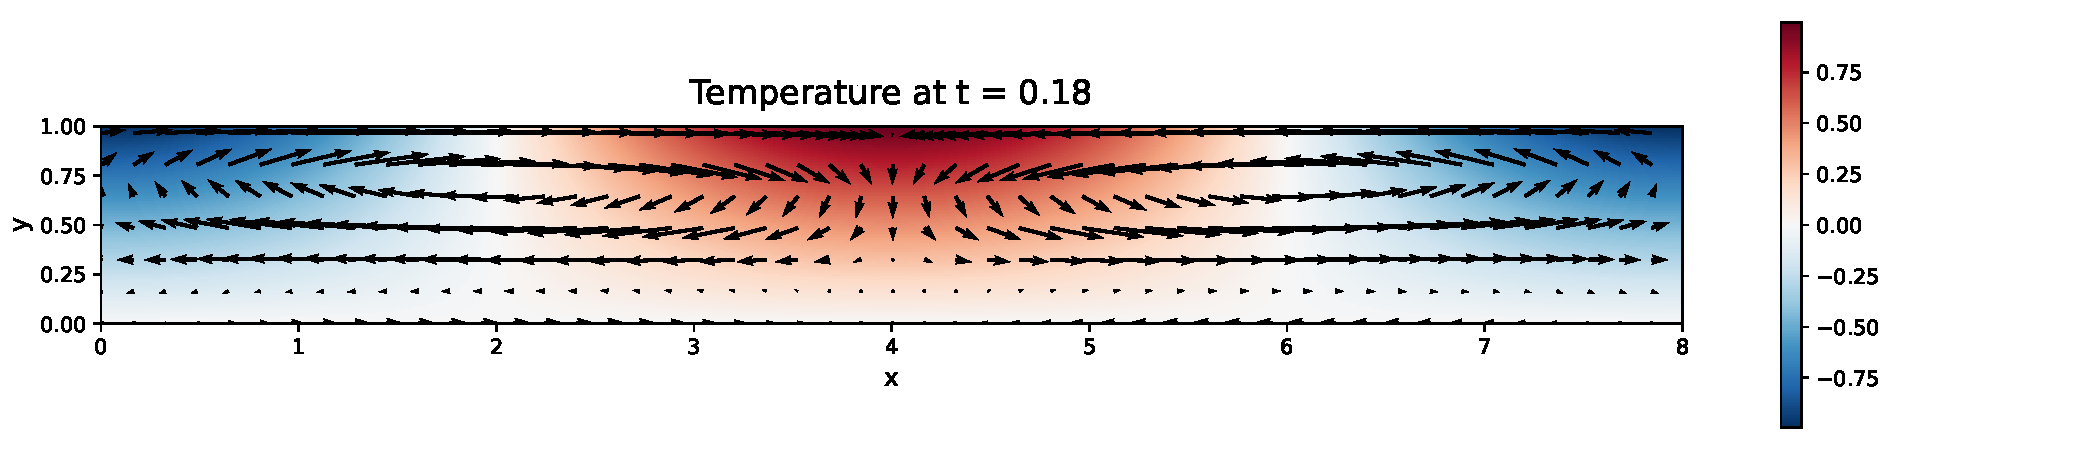
\includegraphics[width=0.75\textwidth]{images/TS_5.pdf}
    \end{subfigure}
    \caption{Transition from a temperature convection to a salinity convection.}
    \label{fig:changeTS}
  \end{figure}

\end{frame}


\begin{frame}{Impact of initial conditions (I)}
  \begin{figure}
    \centering
    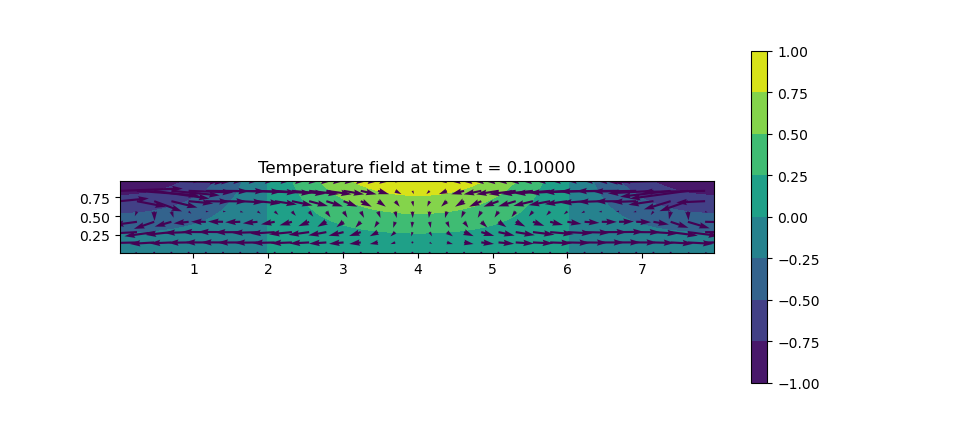
\includegraphics[width=0.8\textwidth]{images/last_subsection/combination_temperature_temp_R_rho_5_to_1_prs_0_1.png}
    \caption{Simulation of the system $(R_{\rho},Le) = (1,10)$ with initial condition $(R_{\rho},Le) = (5,10)$.}
  \end{figure}
\end{frame}

\begin{frame}{Impact of initial conditions (II)}
    
\end{frame}
\section{Conclusions}

\begin{frame}{Conclusions}

\end{frame}


\end{document}



